\section{Algorithm Description}
\label{sec:algorithm}

This section describes an algorithm used to repair ill-typed expressions. The algorithm takes as input an ill-typed expression to be repaired, and two tuning parameters used to guide the internal queries: $N$, the number of possible subexpressions to consider for any type, and $L$, the maximum allowable cost for an expression to be returned. These bounds are necessary to avoid entering an infinitely-deep recursion -- it is not uncommon for classes to accept instances of themselves -- and to control the runtime of the algorithm. \ourTool has access to the environment via the \textit{synthesis graph}, which should be precomputed for libraries, and extended as necessary in an IDE setting.

As a subroutine, \ourTool uses a graph-search-based algorithm for expression synthesis. This portion of the algorithm is of independent value, and can be called directly using our tool.

\subsection{Synthesis Graph Construction}
\label{sec:algorithm:graph}

The data structure central to \ourTool is a colored, directed, weighted, simple bipartite graph $G = (V = V_t \cup V_m, E, w, c)$ between \textit{type} nodes ($V_t$) and \textit{map} nodes ($V_m$), henceforth the \textit{synthesis graph}. A type is any concrete data type, and a map is any language entity that produces exactly one such data type (possibly void) from zero or more types, i.e. it can be modeled by some map $f : (\tau_1 \times \cdots \times \tau_k) \to \sigma$. In the synthesis graph, for each map, an incoming edge is drawn from its co-domain, and outgoing edges are drawn from the map to each type in its domain. These relationships capture the notions that each type or map can be \textit{constructed from} or \textit{satisfied by} other maps or types, respectively.

The weights on the synthesis graph represent the \textit{cost} incurred by including the edge as a part of a candidate snippet. These costs can be derived according to simple heuristics, or computed by examining the frequency of usage over a large corpus. It is important only that no negative costs be assigned anywhere in the graph, and that methods that are more important are valued more than those that are not. The algorithm evaluates candidate expressions by considering their \textit{cost}, not their \textit{value}, so lower edge costs are considered better. Lastly, the synthesis graph is colored according to which language structure added the node to the graph, e.g. constructors, methods, public fields, and the like. These groups color the graph, and are used by the synthesis procedure to decide how to construct the code snippets that ultimately serve as output.

Figure \ref{examplegraph} illustrates a neighborhood of the graph around BufferedReader, a common Java class.

\begin{figure}[!htb]
\centering
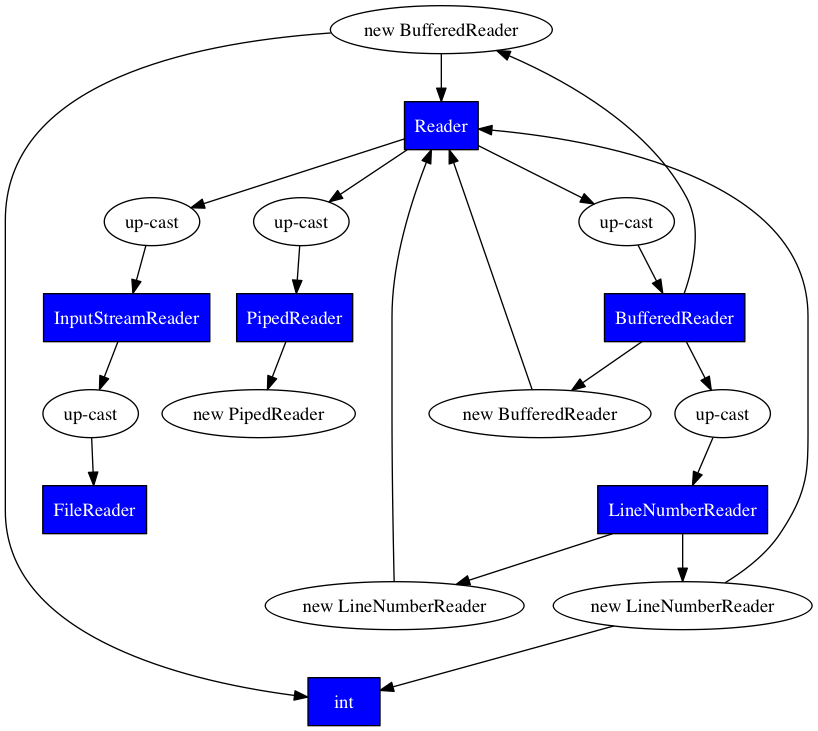
\includegraphics[width=\linewidth]{exampleGraph}
\caption{A subset of a ball of cost-radius $3$ surrounding \texttt{BufferedReader}. The path to \texttt{PipedReader} forms the only valid expression derivable from this graph. The boxed nodes are types, while the ovular nodes are maps.\label{examplegraph}}
\end{figure}

\subsection{Type Inference}

Since it is often the case that very general types, such as integers and strings, carry additional meaning, the synthesis graph must be extended to include abstract type information that encodes whether a particular argument is, for example, a counter, a file descriptor, or an untyped enumeration, in the case of an integer, or in the case of a string, a URL, a file name, or a regular expression. There are already standard approaches for doing this; Lackwit is such a tool for C language programs \cite{DBLP:conf/icse/OCallahanJ97}. Once the abstract types have been identified, they can be added to the graph as subtypes of \texttt{String}, \texttt{int}, etc., with a small, but non-zero cost for ``downcasting'' a normal string or integer to the specific abstract type. This penalty ensures that those expressions that respect the abstract types are preferred over those that don't.

Although this is technically an optional step in so far as it does not pose a challenge to correctness, it serves as a highly-effective heuristic for guiding the search. Even though the returned expressions are always correctly-typed, they might still throw runtime errors; the additional type information recovered by this step reduces the chance of that happening.

\subsection{Synthesis Procedure}

Using this graph, we can answer type-inhabitation queries. That is, given a type $\tau$, we seek expressions of that type that are of low cost. Naturally, we have set the costs so that those expressions that are most desirable are found early on by the algorithm. The \ref{proc:synthesize} procedure, outlined below, answers these queries.

The method proceeds by growing a Dijkstra shortest path ball in the graph of a specified size. This parameter, $L$, acts as a cost limit for the search, and can be tuned to provide a reasonable balance between speed and accuracy, depending on the chosen valuation scheme. The induced subgraph over those nodes is then recursively searched for type satisfaction by \ref{proc:getExpression}, which is called \textit{leaves-first} to enable memoization of its results. Since each type is passed a limit equal to the greatest possible remaining cost during a search from $\tau$, the whole (reduced) space of results is considered for each type. Once a type is settled, the result is added to a memoization table to speed up future calls.

The other tuning parameter, $N$, can be provided to bound both the total number of expressions returned and the number of intermediate results at any given depth by $N$. Because all of the possible generators are considered regardless, we can be sure that the algorithm does not miss any possibilities during the search that might appear among the $N$ best results.

\SetKw{KwNew}{new}
\SetKw{KwIn}{in}
\SetKw{KwNot}{not}
\SetKw{KwWhere}{where}
\SetKw{KwContinue}{continue}
\begin{procedure}
$(V_t\cup V_m, E, w, c)$ $\leftarrow$ $G$ \;
$(D_t, D_m)$ $\leftarrow$ nodes distance less than $L$ away from $\tau\in V_t$\;
\tcc{$D_t, D_m$ ascending by Dijkstra's}
genTable $\leftarrow$ $\left\{\left\{\right\}\right\}$ \;
snippetTable $\leftarrow$ $\left\{\left\{\right\}\right\}$ \;
\ForEach{$(f : (\tau_1 \times \cdots \times \tau_k) \to \sigma) \in D_m$}{
	\tcc{Keep only the best $N$ elements}
	genTable[$\tau$] $\leftarrow$ genTable[$\tau$] $\cup$ $\{(f, w(f))\}$ \;
}
typeStack $\leftarrow$ \KwNew Stack\;
\ForEach{$\sigma \in D_t$}{
	push $(\sigma, L-\text{shortestPathLength}(\sigma))$ on to typeStack\;
}
\While{typeStack is not empty}{
	$(\sigma, l)$ $\leftarrow$ pop typeStack \;
	snippetTable[$\sigma$] $\leftarrow$ \ref{proc:getExpression}(genTable, snippetTable, $\sigma$, $l$, $N$) \;
}
\Return{snippetTable[$\tau$]}\;
\caption{Synthesize($G$, $\tau$, $L$, $N$)}\label{proc:synthesize}
\end{procedure}

Note that in \ref{proc:synthesize}, all sets are maintained in sorted order using a tree data structure, and \textit{genTable} and \textit{snippetTable} are both hash tables of these sets.

Once the results from \ref{proc:synthesize} have been obtained, the built up expressions can be converted into strings by recursively applying a string formatting function appropriate for the colors of each generator in the expression. The leaves ($0$-input maps) evaluate to known strings, and fill in the parameters of the maps above them until a complete code snippet is built.

The subroutine \ref{proc:getExpression} goes through each possible generator for a given type and attempts to satisfy its argument types recursively. It checks a memoization table before computing the set of expressions to avoid repeating work. The recursion itself is straight-forward: for each function that can generate the requested type, attempt to satisfy all of its parameters, add all those whose parameters were satisfied and whose total cost is beneath the limit $L$, keeping only the best $N$ encountered.
\begin{procedure}
\lIf{$\tau$ $\in$ snipT}{\Return{snipT[$\tau$]}}
snips $\leftarrow$ $\{\}$ \; \label{proc:getExpression:snipInit}
gens $\leftarrow$ genT[$\sigma$] \;
\ForEach{$(f : (\tau_1 \times \cdots \times \tau_k) \to \sigma, w')$ $\in$ gens}{
	\lIf{$w' > L$}{\KwContinue}
	$s_i$ $\leftarrow$ \ref{proc:getExpression}(genT, snipT, $\tau_i$, $L - w'$, $N$) $\forall i$\;
	\ForEach{args $\in$ $s_1 \times \cdots \times s_k$}{
		cost $\leftarrow$ $w' + \sum_{i=1}^{k} w(args[i])$ \; \label{proc:getExpression:cost}
		exp $\leftarrow$ $(f(args), cost)$ \;
		\If{cost $\leq L \wedge | \text{snips} | < N$}{
			snips $\leftarrow$ snips $\cup$ $\{$ exp $\}$ \;
		}
		\ElseIf{cost $\leq L \wedge | \text{snips} | = N$}{
			$e'=(maxE, maxCost)$ $\leftarrow$ popMax(snips) \;
			snips $\leftarrow$ snips $\cup$ $\{$ min($e'$, exp) $\}$
		}
	}
}
\Return{snippets}
\caption{GetExpressions(genT, snipT, $\sigma$, $L$, $N$)}\label{proc:getExpression}
\end{procedure}

\subsection{Repair Procedure}
We are now ready to describe the repair procedure. The key step in our approach is biasing the synthesis towards those subexpressions of the backbone expression that are, in fact, correctly-typed. The reasoning behind this is intuitive; if a user specifies that she would like to create a new type from some specific components, the search should be optimized to favor using those same components.

To do this, we modify the \ref{proc:getExpression} procedure to accept a preference map, \textit{pref}, supplied by the repair procedure. The preference map contains a set of subexpressions (indexed by their type) which will be used to bias the search in their favor. We modify \ref{proc:getExpression} so that line \ref{proc:getExpression:snipInit} initializes \textit{snips} with \textit{pref[$\tau$]}, rather than the empty set, and line \ref{proc:getExpression:cost} reduces the cost of each result by a factor of $2^{n}$, where $n$ is the number of expressions in the preference map which occur in $f(args)$. Since \ref{proc:getExpression} is a subroutine of \ref{proc:synthesize}, we must add an argument to its signature in order to forward the preference map to \ref{proc:getExpression}.

This scheme has a few distinct advantages: first, it will very strongly prefer those expressions that occurred as part of the given incorrect expression; second, in cases where more than one element of the same type is required, it will favor diversity over homogeneity (ie. if both $a$ and $b$ were specified, it will try to use both); and finally, if no subexpressions are supplied, then the modified algorithm degenerates into its original form.

With this modification in place, the repair algorithm proceeds from the bottom up. When we insert an expression  in to \textit{pref}, we will say that we have \textit{enforced} that expression. So, for each broken subexpression in the backbone, we first enforce all of its correctly-typed child expressions and then initiate a synthesis on the current subexpression. If any of its children are not correctly typed, we recurse and repair them first.

Notice that this means the repaired subexpressions will also be enforced. This behavior is desirable since it favors reusing the computations made before when synthesis occurs at a higher level. Additionally, this process  only enforces those literals that are contained within a given subexpression, so that two disjoint subexpressions do not interfere while initiating a nested repair.

\begin{procedure}
\lIf{expr is well-typed}{\Return{(expr, $\{\}$)}}
$f: (x_1: \tau_1, \ldots, x_k: \tau_k): \sigma$ $\leftarrow$ expr\;
\tcc{$S$ is the preference map}
$S \leftarrow \{\}$ \;
\ForEach{$x \in \{x_1,\ldots,x_k\}$}{
	$(x, S_x) \leftarrow$ \ref{proc:repair}($x$, $L$, $N$)\;
	$S \leftarrow S \cup S_x$ \;
}
$S \leftarrow S \cup \{x_1,\ldots,x_k\}$ \;
\tcc{enforce $S$ via fifth argument}
\Return{(\ref{proc:synthesize}($G$, $\sigma$, $L$, $N$, $S$), $S$)}
\caption{Repair($G$, expr, $L$, $N$)}\label{proc:repair}
\end{procedure}

\lipsum[1-24]
